\documentclass[11pt,a4paper]{article}

\usepackage[T1]{fontenc}
\usepackage[utf8]{inputenc}
\usepackage[margin=25mm]{geometry}
\usepackage{amsmath}
\usepackage{amssymb}
\usepackage{siunitx}
\usepackage{booktabs}
\usepackage{graphicx}
\usepackage{circuitikz}
\usepackage{pgfplots}
\pgfplotsset{compat=1.15}

\sisetup{output-decimal-marker={.},per-mode=symbol}

\title{The EPCOS SIOV-B80K680 Block Varistor:\\
Operating Characteristics and Application Sizing}
\author{Davide Bagnara}
\date{\today}

\begin{document}
\maketitle

\begin{abstract}
This note describes the operating characteristics of the EPCOS SIOV-B80K680
metal-oxide block varistor (HighE series) starting from the manufacturer
datasheet, derives an analytical model of its $V$--$I$ characteristic, and
develops a complete sizing example: line-side overvoltage protection of a
high-power thyristor converter fed from a \SI{600}{\volt} industrial network.
The sizing covers the continuous operating voltage, the protection level and
its coordination with the semiconductor blocking voltage, the single-pulse
energy capability, and the average-power (repetition-rate) limit. A custom
Simscape implementation of the device model is described and verified
against the datasheet points.
\end{abstract}

\section{Introduction}

A metal-oxide varistor (MOV) is a voltage-dependent resistor based on
sintered zinc-oxide (ZnO) ceramic. The ZnO grains are good conductors, while
the grain boundaries behave as back-to-back Schottky-like barriers with a
breakdown voltage of roughly \SI{3.5}{\volt} each. A varistor disk is
therefore electrically equivalent to a large series--parallel network of
microvaristors: the disk thickness sets the varistor voltage, the disk area
sets the current and energy capability. This is why, within the same voltage
class, the EPCOS HighE series scales from the B32 (\SI{32}{\milli\meter}
disk) up to the B80 (\SI{80}{\milli\meter} disk) with surge current ratings
from \SI{25}{\kilo\ampere} to \SI{100}{\kilo\ampere}~\cite{epcos2002,epcos_gti}.

The resulting terminal behavior is a strongly nonlinear, symmetric $V$--$I$
characteristic, commonly approximated by the power law
%
\begin{equation}
  i = k\,v^{\alpha},
  \label{eq:powerlaw}
\end{equation}
%
with a nonlinearity exponent $\alpha$ in the range 25--40 for ZnO. Three
regions can be identified:
%
\begin{enumerate}
  \item \emph{Leakage region} (below the varistor voltage): the device is
  essentially a capacitor with a small, temperature-dependent resistive
  leakage current;
  \item \emph{Normal operation (clamping) region}: the grain-boundary
  barriers conduct and the power law \eqref{eq:powerlaw} holds; the voltage
  rises only weakly with current;
  \item \emph{Upturn region} (tens of \si{\kilo\ampere}): the bulk resistance
  of the ZnO grains dominates and the characteristic becomes nearly ohmic.
\end{enumerate}

The B80K680 is the \SI{80}{\milli\meter} disk of the \SI{680}{\volt} (AC)
voltage class, i.e.\ the largest energy-handling member of its class in the
HighE family, intended for heavy-duty protection of low-voltage industrial
equipment: converter inputs, large drives, distribution panels and
machine-tool supplies.

\section{Datasheet Data}

Table~\ref{tab:data} collects the ratings and characteristics of the
B80K680~\cite{epcos2002}.

\begin{table}[htb]
\centering
\caption{SIOV-B80K680 ratings ($T_A = \SI{85}{\celsius}$) and
characteristics ($T_A = \SI{25}{\celsius}$).}
\label{tab:data}
\begin{tabular}{lll}
\toprule
Quantity & Symbol & Value \\
\midrule
Max.\ continuous AC voltage & $V_\mathrm{RMS}$ & \SI{680}{\volt} \\
Max.\ continuous DC voltage & $V_\mathrm{DC}$ & \SI{895}{\volt} \\
Max.\ surge current (8/20~\si{\micro\second}, single pulse) & $i_\mathrm{max}$ & \SI{100}{\kilo\ampere} \\
Max.\ single-pulse energy (\SI{2}{\milli\second}) & $W_\mathrm{max}$ & \SI{3600}{\joule} \\
Max.\ average power dissipation & $P_\mathrm{max}$ & \SI{2.0}{\watt} \\
Varistor voltage at \SI{1}{\milli\ampere} (DC) & $V_v$ & \SI{1100}{\volt} $\pm\,10\,\%$ \\
Max.\ clamping voltage at \SI{800}{\ampere} (8/20~\si{\micro\second}) & $v_c$ & \SI{1815}{\volt} \\
Typical capacitance (\SI{1}{\kilo\hertz}) & $C_\mathrm{typ}$ & \SI{5200}{\pico\farad} \\
Response time & & $< \SI{25}{\nano\second}$ \\
Operating temperature & & \SIrange{-40}{85}{\celsius} \\
Electric strength (housing) & & $\geq \SI{2.5}{\kilo\volt}$ RMS \\
Terminals / max.\ torque & & M5 / \SI{2.5}{\newton\meter} \\
Weight & & approx.\ \SI{650}{\gram} \\
\bottomrule
\end{tabular}
\end{table}

Two remarks on these figures:
%
\begin{itemize}
  \item The energy rating $W_\mathrm{max}$ refers to a \emph{single}
  \SI{2}{\milli\second} rectangular pulse. Repetitive surges must be checked
  against the derating curves of the datasheet, which trade pulse amplitude
  and duration against the admissible number of pulses over the device
  lifetime.
  \item $P_\mathrm{max}$ is a thermal steady-state limit: it bounds the
  \emph{average} dissipation (standby losses plus the time-averaged surge
  energy) so that the disk temperature, and hence the leakage current,
  remains stable. ZnO leakage has a negative temperature coefficient, so
  exceeding $P_\mathrm{max}$ can trigger thermal runaway.
\end{itemize}

\section{Analytical $V$--$I$ Model}

The datasheet provides two points of the characteristic: the varistor
voltage $(\SI{1}{\milli\ampere},\,\SI{1100}{\volt})$ and the clamping point
$(\SI{800}{\ampere},\,\SI{1815}{\volt})$. Fitting the power law
\eqref{eq:powerlaw} through both points gives the nonlinearity exponent
%
\begin{equation}
  \alpha
  = \frac{\ln(i_2/i_1)}{\ln(v_2/v_1)}
  = \frac{\ln\!\left(800/10^{-3}\right)}{\ln\!\left(1815/1100\right)}
  = \frac{13.59}{0.501}
  \approx 27.1 ,
\end{equation}
%
a typical value for ZnO. Inverting \eqref{eq:powerlaw}, the clamping voltage
as a function of current is
%
\begin{equation}
  v = C\, i^{\beta},
  \qquad
  \beta = \frac{1}{\alpha} \approx 0.0369,
  \qquad
  C \approx \SI{1419}{\volt} \;\text{(at $i = \SI{1}{\ampere}$)} .
  \label{eq:vofi}
\end{equation}
%
Equation \eqref{eq:vofi} reproduces both datasheet points within
\SI{0.2}{\percent} and is plotted in Fig.~\ref{fig:vi}. It is valid between
the two fitting points; extrapolation towards the surge-current range
(above a few \si{\kilo\ampere}) underestimates the upturn caused by the
grain bulk resistance and should be replaced by the datasheet $V/I$ curves
for accurate coordination studies.

\begin{figure}[htb]
\centering
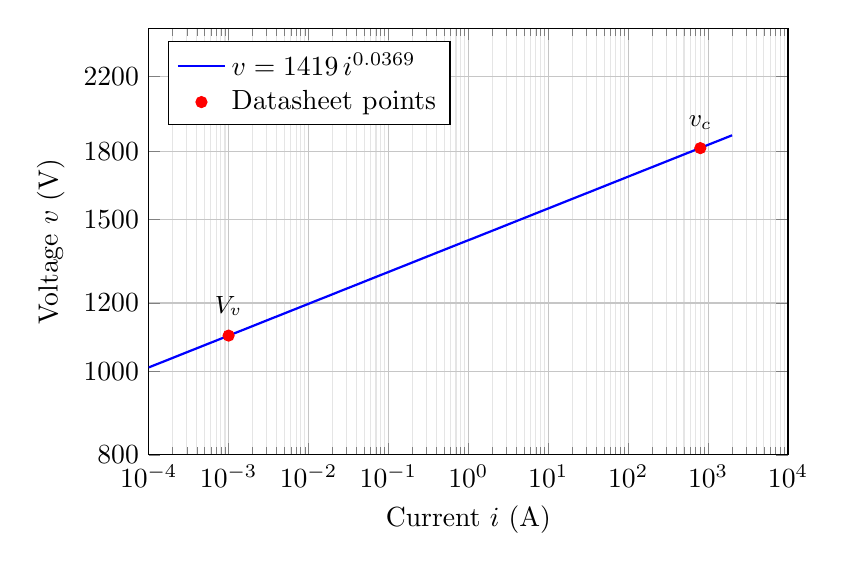
\begin{tikzpicture}
\begin{loglogaxis}[
  width=0.8\textwidth,
  height=7cm,
  xlabel={Current $i$ (\si{\ampere})},
  ylabel={Voltage $v$ (\si{\volt})},
  xmin=1e-4, xmax=1e4,
  ymin=800, ymax=2500,
  ytick={800,1000,1200,1500,1800,2200},
  yticklabels={800,1000,1200,1500,1800,2200},
  grid=both,
  minor grid style={gray!20},
  major grid style={gray!45},
  legend pos=north west,
  legend cell align=left,
]
\addplot[blue, thick, domain=1e-4:2e3, samples=100]
  {1419*x^0.0369};
\addlegendentry{$v = 1419\, i^{0.0369}$}
\addplot[only marks, mark=*, red] coordinates {(1e-3,1100) (800,1815)};
\addlegendentry{Datasheet points}
\node[anchor=south, font=\small] at (axis cs:1e-3,1130) {$V_v$};
\node[anchor=south, font=\small] at (axis cs:800,1860) {$v_c$};
\end{loglogaxis}
\end{tikzpicture}
\caption{Fitted $V$--$I$ characteristic of the B80K680 (clamping region).}
\label{fig:vi}
\end{figure}

\subsection{Capacitance and standby behavior}

With $C_\mathrm{typ} = \SI{5200}{\pico\farad}$, the capacitive reactance at
\SI{50}{\hertz} is
%
\begin{equation}
  X_C = \frac{1}{2\pi \cdot 50 \cdot 5.2\times 10^{-9}}
  \approx \SI{612}{\kilo\ohm},
\end{equation}
%
so at the full rated voltage of \SI{680}{\volt} RMS the capacitive current is
about \SI{1.1}{\milli\ampere} --- comparable to the \SI{1}{\milli\ampere}
resistive reference current that defines $V_v$. At mains frequency the
standby current of a large-disk varistor is therefore mostly capacitive and
the standby losses remain far below $P_\mathrm{max}$. The same capacitance
must be kept in mind on converter terminals with high $\mathrm{d}v/\mathrm{d}t$:
\SI{5.2}{\nano\farad} across a switching node is a non-negligible snubber-like
load, which is one reason why block varistors are normally installed on the
line side rather than directly across fast-switching devices.

\section{Application Example: Line-Side Protection of a Thyristor Converter}

\subsection{System description}

Consider a high-power thyristor converter (soft starter or controlled
rectifier, hundreds of \si{\kilo\watt}) fed from a $3\times\SI{600}{\volt}$,
\SI{50}{\hertz} industrial network with $\pm 10\,\%$ voltage tolerance. The
thyristors have a repetitive blocking voltage
$V_\mathrm{DRM} = V_\mathrm{RRM} = \SI{2200}{\volt}$. The installation is
exposed to switching surges (breaker operation on transformers and reactors)
and to induced lightning surges, assumed up to \SI{10}{\kilo\ampere} with
8/20~\si{\micro\second} waveshape. Three varistors are delta-connected at the
converter input terminals (Fig.~\ref{fig:circuit}).

\begin{figure}[htb]
\centering
\begin{circuitikz}[american, scale=0.9, transform shape]
  % Three-phase lines
  \draw (0,4) to[short] (2,4) to[L, l=$L_s$] (4,4) to[short] (9,4);
  \draw (0,2.5) to[short] (2,2.5) to[L, l=$L_s$] (4,2.5) to[short] (9,2.5);
  \draw (0,1) to[short] (2,1) to[L, l=$L_s$] (4,1) to[short] (9,1);
  \node[anchor=east] at (0,4) {L1};
  \node[anchor=east] at (0,2.5) {L2};
  \node[anchor=east] at (0,1) {L3};
  % Delta-connected varistors
  \draw (5.3,4) to[varistor, l_=$R_{V12}$] (5.3,2.5);
  \draw (6.5,2.5) to[varistor, l_=$R_{V23}$] (6.5,1);
  % RV31 from L1 to L3 with a hop over L2
  \draw (7.7,4) to[varistor, l=$R_{V31}$] (7.7,2.62);
  \draw (7.7,2.62) arc[start angle=90, end angle=-90, radius=0.12];
  \draw (7.7,2.38) -- (7.7,1);
  \draw (5.3,4) node[circ]{};
  \draw (5.3,2.5) node[circ]{};
  \draw (6.5,2.5) node[circ]{};
  \draw (6.5,1) node[circ]{};
  \draw (7.7,4) node[circ]{};
  \draw (7.7,1) node[circ]{};
  % Converter block
  \draw (9,0.4) rectangle (11,4.6);
  \node[align=center] at (10,2.5) {Thyristor\\converter};
\end{circuitikz}
\caption{Delta-connected B80K680 varistors at the input of a thyristor
converter. $L_s$ is the source (line/transformer) inductance.}
\label{fig:circuit}
\end{figure}

\subsection{Step 1: continuous operating voltage}

For line-to-line connection the varistor sees, in the worst case,
%
\begin{equation}
  V_\mathrm{LL,max} = 1.1 \cdot \SI{600}{\volt} = \SI{660}{\volt}
  \;\leq\; V_\mathrm{RMS} = \SI{680}{\volt} \quad \checkmark
\end{equation}
%
A useful additional check is that the network crest voltage never enters the
conduction region even for the worst-case tolerance of the varistor voltage
($-10\,\%$, i.e.\ $V_{v,\min} = \SI{990}{\volt}$):
%
\begin{equation}
  \hat v = \sqrt{2}\cdot \SI{660}{\volt} = \SI{933}{\volt}
  \;<\; V_{v,\min} = \SI{990}{\volt} \quad \checkmark
\end{equation}
%
so the resistive standby current stays below the \SI{1}{\milli\ampere}
reference level at every point of the mains cycle. Note that the
\SI{680}{\volt} class is the correct choice for a \SI{600}{\volt} network;
on a \SI{690}{\volt} network ($+10\,\% \rightarrow \SI{759}{\volt}$) the
next class up (K750) would be required.

\subsection{Step 2: protection level and coordination}

At the tabulated clamping point the varistor limits the terminal voltage to
$v_c = \SI{1815}{\volt}$ at \SI{800}{\ampere}. The coordination margin with
respect to the thyristor blocking voltage is
%
\begin{equation}
  \frac{V_\mathrm{DRM}}{v_c} = \frac{2200}{1815} \approx 1.21 ,
\end{equation}
%
i.e.\ about \SI{20}{\percent}, which is the usual minimum for insulation
coordination. Two practical caveats:
%
\begin{itemize}
  \item For the assumed \SI{10}{\kilo\ampere} surge, the model
  \eqref{eq:vofi} extrapolates to $v \approx \SI{2.0}{\kilo\volt}$, and the
  real curve (upturn region) is somewhat higher. The residual margin at full
  surge current is therefore thin: the datasheet $V/I$ curve (page 285
  of~\cite{epcos2002}) must be used for the final check, and this is
  precisely the reason to select the largest disk (B80) of the voltage
  class --- for a given current, a larger disk clamps at a lower voltage.
  \item The connection inductance adds $L\,\mathrm{d}i/\mathrm{d}t$ to the
  clamping voltage seen by the converter. With the 8/20~\si{\micro\second}
  front ($\mathrm{d}i/\mathrm{d}t \approx \SI{1.25}{\kilo\ampere\per\micro\second}$
  at \SI{10}{\kilo\ampere}) each meter of loop (\(\approx\SI{1}{\micro\henry}\))
  adds about \SI{1.25}{\kilo\volt}. Varistor leads must be as short as
  possible and the varistor connected directly at the terminals to be
  protected.
\end{itemize}

\subsection{Step 3: surge current and energy}

\paragraph{Lightning-type surge.}
For a \SI{10}{\kilo\ampere}, 8/20~\si{\micro\second} pulse the absorbed
energy can be bounded conservatively with an equivalent duration of
\SI{20}{\micro\second}:
%
\begin{equation}
  W_\mathrm{surge} \approx v_c \, \hat\imath \, t_\mathrm{eq}
  \approx \SI{2000}{\volt} \cdot \SI{10}{\kilo\ampere} \cdot
  \SI{20}{\micro\second} = \SI{400}{\joule}
  \;\ll\; W_\mathrm{max} = \SI{3600}{\joule} \quad \checkmark
\end{equation}
%
The peak current itself is far below the single-pulse rating
($\SI{10}{\kilo\ampere} \ll \SI{100}{\kilo\ampere}$); for the expected
number of surges over the equipment lifetime the admissible amplitude is
read from the derating curve (page 264 of~\cite{epcos2002}).

\paragraph{Inductive energy dump.}
The dimensioning event for the energy rating is usually not the lightning
surge but the interruption of an inductive current: when the line breaker
clears, the magnetic energy stored in the source and smoothing inductances
is transferred to the varistors. Assuming the breaker interrupts
$I_0 = \SI{1.2}{\kilo\ampere}$ flowing in a total commutation/smoothing
inductance $L = \SI{1.5}{\milli\henry}$:
%
\begin{equation}
  W_L = \tfrac{1}{2} L I_0^2
      = \tfrac{1}{2}\cdot\SI{1.5}{\milli\henry}\cdot(\SI{1.2}{\kilo\ampere})^2
      = \SI{1080}{\joule}
  \;=\; 0.30\, W_\mathrm{max} \quad \checkmark
\end{equation}
%
During the dump the varistor clamps at
$v \approx 1419\cdot 1200^{0.0369} \approx \SI{1.84}{\kilo\volt}$
(from \eqref{eq:vofi}), still coordinated with the thyristors, and the
current decays approximately linearly in
$t \approx L I_0 / v_c \approx \SI{1}{\milli\second}$, consistent with the
\SI{2}{\milli\second} basis of the energy rating.

\subsection{Step 4: average power and repetition rate}

After a full \SI{1080}{\joule} event the device needs a cool-down interval
of at least
%
\begin{equation}
  t_\mathrm{rep} \geq \frac{W_L}{P_\mathrm{max}}
  = \frac{1080}{2.0} = \SI{540}{\second} ,
\end{equation}
%
i.e.\ roughly one energy dump every ten minutes in continuous service. If
the protection concept requires more frequent operations (e.g.\ a
load-commutation duty rather than an emergency clamp), the varistor is the
wrong device and an active clamp or a braking chopper must absorb the
energy, with the varistor kept as last-resort protection only.

\subsection{Result}

A single B80K680 per phase pair (three devices, delta connection) satisfies
all four checks for the \SI{600}{\volt} converter: continuous voltage margin
\SI{3}{\percent} at $+10\,\%$ grid tolerance, protection ratio 1.21 at the
tabulated clamping point, single-pulse energy utilization \SI{30}{\percent},
and a repetition capability of one full dump per \SI{540}{\second}. The
tight coordination margin at \SI{10}{\kilo\ampere} is the critical item and
must be verified on the datasheet $V/I$ curve; if the margin proves
insufficient, the options are a higher thyristor blocking class or a hybrid
scheme (varistor plus RC snubber to slow the front).

\section{Practical Notes}

\begin{itemize}
  \item \emph{End-of-life behavior.} A varistor degraded by repeated surges
  fails towards lower varistor voltage and eventually to a short circuit.
  Each device should be protected by a fuse or thermal disconnector able to
  clear the resulting fault current, and its state should be monitored
  (visual indicator or supervision contact) in permanently installed
  equipment.
  \item \emph{Paralleling.} Because of the steep characteristic
  ($\alpha \approx 27$), small differences in $V_v$ cause large current
  imbalance between paralleled varistors. Paralleling requires devices
  matched in $V_v$; it is generally preferable to select a single larger
  disk, which is exactly the role of the B80 size.
  \item \emph{Mounting.} M5 screw terminals, max.\ torque
  \SI{2.5}{\newton\meter}; the potted housing withstands
  $\geq\SI{2.5}{\kilo\volt}$ RMS to the mounting surface, but creepage and
  clearance of the external connections must still be verified for the
  \SI{600}{\volt} network (overvoltage category and pollution degree of the
  installation).
  \item \emph{Temperature.} All ratings of Table~\ref{tab:data} hold up to
  $T_A = \SI{85}{\celsius}$; above that, voltage and energy must be derated
  per the datasheet derating curves.
\end{itemize}

\section{Simscape Implementation}
\label{sec:simscape}

The device is implemented as a custom Simscape language component
(\texttt{varistor\_mov.ssc}) for the personal component library, so that it
can be used in circuit simulations without requiring Simscape Electrical.
Its default parameterization is the B80K680.

\subsection{Equivalent circuit and equations}

The model structure is shown in Fig.~\ref{fig:sscmodel}: a series inductance
$L_s$ and bulk resistance $R_b$ feed the ZnO core, modeled as the parallel
combination of the nonlinear resistor $R_\mathrm{nl}$, the leakage
resistance $R_p$ and the capacitance $C$.

\begin{figure}[htb]
\centering
\begin{circuitikz}[american]
  \draw (0,0) node[ocirc]{} node[above]{$p$}
    to[L, l=$L_s$, i=$i$] (2,0)
    to[R, l=$R_b$] (4,0) -- (7.6,0);
  \draw (4.6,0) to[varistor, l_=$R_\mathrm{nl}$] (4.6,-2.4);
  \draw (6.1,0) to[R, l_=$R_p$] (6.1,-2.4);
  \draw (7.6,0) to[C, l=$C$] (7.6,-2.4);
  \draw[-latex] (6.85,-2.0) -- (6.85,-0.4);
  \node[right] at (6.85,-1.2) {$v_c$};
  \draw (4.6,-2.4) -- (7.6,-2.4) -- (8.8,-2.4) node[ocirc]{} node[above]{$n$};
  \draw (4.6,0) node[circ]{};
  \draw (6.1,0) node[circ]{};
  \draw (6.1,-2.4) node[circ]{};
\end{circuitikz}
\caption{Structure of the Simscape varistor model.}
\label{fig:sscmodel}
\end{figure}

The governing equations are
%
\begin{align}
  v &= L_s \frac{\mathrm{d}i}{\mathrm{d}t} + R_b\, i + v_c ,
  \label{eq:ssc-terminal}\\[2pt]
  i &= C \frac{\mathrm{d}v_c}{\mathrm{d}t} + i_\mathrm{nl}
       + \frac{v_c}{R_p} ,
  \label{eq:ssc-node}\\[2pt]
  i_\mathrm{nl} &= I_1 \, \frac{v_c}{V_1}
    \left( \frac{|v_c|}{V_1} \right)^{\alpha - 1},
  \qquad
  \alpha = \frac{\ln (I_2/I_1)}{\ln (V_2/V_1)} ,
  \label{eq:ssc-powerlaw}\\[2pt]
  \frac{\mathrm{d}E_\mathrm{abs}}{\mathrm{d}t}
    &= v_c \left( i_\mathrm{nl} + \frac{v_c}{R_p} \right) + R_b\, i^2 .
  \label{eq:ssc-energy}
\end{align}
%
The power law \eqref{eq:ssc-powerlaw} is written in odd-symmetric form,
$v_c \, |v_c|^{\alpha-1}$, which avoids the discontinuous
$\operatorname{sign}(\cdot)$ function and is differentiable at
$v_c = 0$ --- no zero-crossing events are generated. The component is
parameterized directly with the two datasheet points $(V_1, I_1)$ and
$(V_2, I_2)$, and $\alpha$ is computed internally per
\eqref{eq:ssc-powerlaw}, exactly as in Section~3; no derived parameter has
to be entered by hand. The three characteristic regions map onto the three
core branches: $R_p$ covers the leakage region (where the bare power law
underestimates the real leakage current), the power law covers the clamping
region (exact at the two fit points), and $R_b$ approximates the upturn
region.

Equation \eqref{eq:ssc-energy} integrates the \emph{dissipated} energy only
(core plus $R_b$, excluding the energy stored in $C$), so that
$E_\mathrm{abs}$ is directly comparable with the single-pulse rating
$W_\mathrm{max}$ of Table~\ref{tab:data}. An optional runtime assertion
stops the simulation when $E_\mathrm{abs} > W_\mathrm{max}$; since the
integral is cumulative, the check is meaningful for single-event
simulations.

\subsection{Parameters}

Table~\ref{tab:sscpar} lists the model parameters with their B80K680
default values.

\begin{table}[htb]
\centering
\caption{Parameters of \texttt{varistor\_mov} (defaults: B80K680).}
\label{tab:sscpar}
\begin{tabular}{llll}
\toprule
Parameter & Default & Source & Role \\
\midrule
$V_1$, $I_1$ & \SI{1100}{\volt}, \SI{1}{\milli\ampere} & datasheet & varistor voltage point \\
$V_2$, $I_2$ & \SI{1815}{\volt}, \SI{800}{\ampere} & datasheet & clamping point \\
$C$ & \SI{5200}{\pico\farad} & datasheet & core capacitance \\
$R_p$ & \SI{100}{\mega\ohm} & assumed & leakage region \\
$R_b$ & \SI{1}{\milli\ohm} & placeholder & upturn region \\
$L_s$ & \SI{50}{\nano\henry} & estimated & element + terminals \\
$W_\mathrm{max}$ & \SI{3600}{\joule} & datasheet & energy assertion limit \\
\bottomrule
\end{tabular}
\end{table}

Two parameters deserve comment. $R_b$ is a placeholder: with
\SI{1}{\milli\ohm} it adds only \SI{100}{\volt} at \SI{100}{\kilo\ampere},
so if surge currents above roughly \SI{10}{\kilo\ampere} matter, $R_b$
should be refitted on the upper part of the datasheet $V/I$ curve.
$L_s$ must be kept strictly positive: it defines the current state of the
component (with $L_s = 0$ equation \eqref{eq:ssc-terminal} degenerates into
an algebraic constraint and the DAE index increases), and it represents in
any case the physical inductance of the element and its terminals; external
lead inductance is added in the surrounding circuit.

\subsection{Verification and numerical remarks}

Solving \eqref{eq:ssc-terminal}--\eqref{eq:ssc-powerlaw} at DC reproduces
the datasheet points: $v(\SI{1}{\milli\ampere}) = \SI{1099.6}{\volt}$ and
$v(\SI{800}{\ampere}) = \SI{1815.8}{\volt}$, where the residuals of about
\SI{1}{\volt} are the $R_b$ and $R_p$ contributions. At
\SI{10}{\kilo\ampere} the model gives $v \approx \SI{2.0}{\kilo\volt}$,
consistent with the extrapolation discussed in Section~4.2 (and subject to
the same caveat on the upturn region). At the network crest voltage of the
sizing example (\SI{933}{\volt}) the resistive standby current is
\SI{21}{\micro\ampere}, dominated by the $R_p$ branch, confirming that at
mains frequency the terminal current is essentially capacitive.

With $\alpha \approx 27$ the model is numerically stiff: the incremental
resistance of the core spans more than eight decades between standby and
clamping. A stiff solver (\texttt{ode23t} or \texttt{ode15s}) should be
used, as for the other nonlinear device models of the library.



The B80K680 combines a \SI{680}{\volt} continuous AC rating with
\SI{100}{\kilo\ampere} surge capability and \SI{3600}{\joule} single-pulse
energy, making it suitable as heavy-duty line-side protection for
\SI{600}{\volt}-class power converters. A two-point power-law fit of the
datasheet characteristic ($\alpha \approx 27$,
$v \approx 1419\,i^{0.0369}$) is sufficient for first-pass sizing of the
clamping voltage and of the energy absorbed in inductive dump events, while
the final coordination at full surge current must rely on the datasheet
$V/I$ and derating curves. In the worked example the device passes all
sizing checks with the protection-level coordination as the binding
constraint --- the typical situation when protecting \SI{2200}{\volt}
thyristors on a \SI{600}{\volt} network. The same two-point
parameterization drives the custom Simscape component of
Section~\ref{sec:simscape}, which reproduces the datasheet points and makes
the device directly usable in transient circuit simulations.

\begin{thebibliography}{9}

\bibitem{epcos2002}
EPCOS AG, ``Block Varistors, HighE Series,'' SIOV Metal Oxide Varistors
data book, pp.~221--226, Apr.~2002.

\bibitem{epcos_gti}
EPCOS AG, ``SIOV Metal Oxide Varistors --- General Technical Information,''
SIOV data book, 2002.

\bibitem{harnden1972}
J.~D. Harnden, F.~D. Martzloff, W.~G. Morris, and F.~B. Golden,
``Metal-oxide varistor: a new way to suppress transients,''
\emph{Electronics}, vol.~45, no.~21, pp.~91--95, Oct.~1972.

\bibitem{iec61643}
IEC 61643-11, \emph{Low-voltage surge protective devices --- Part 11:
Surge protective devices connected to low-voltage power systems ---
Requirements and test methods}, International Electrotechnical Commission.

\end{thebibliography}

\end{document}
